\hypertarget{ch:hypothesis}{%
\chapter{Hypothesis Testing}\label{ch:hypothesis}}

Hypothesis testing can be thought of as a stochastic analog of proof by
contradiction.

``To understand the essence of statistical hypothesis testing properly, it is
necessary to compare intentionally hypothesis testing with proof by
contradiction and characterize the former as not the same as the latter.''
\citep{otani2019comparing}.

It should be relatively clear, then, why a failure to reject H , does not
constitute a verification of its truth. It simply means that the researcher has
failed to provide evidence suflcient to cast serious doubt on the truth of
\(H_0\). \citep{reeves1980hypothesis}

Misconception \citep{falk1995significance}.

Consider testing whether two sample have the same mean.

\begin{knitrout}
\definecolor{shadecolor}{rgb}{0.969, 0.969, 0.969}\color{fgcolor}\begin{kframe}
\begin{alltt}
\hlkwd{set.seed}\hlstd{(}\hlnum{20210628}\hlstd{)}
\hlstd{delta} \hlkwb{<-} \hlnum{0}
\hlstd{n1} \hlkwb{<-} \hlstd{n2} \hlkwb{<-} \hlstd{n} \hlkwb{<-} \hlnum{30}
\hlstd{x1} \hlkwb{<-} \hlkwd{rnorm}\hlstd{(n)}
\hlstd{x2} \hlkwb{<-} \hlkwd{rnorm}\hlstd{(n2)} \hlopt{+} \hlstd{delta}
\hlkwd{t.test}\hlstd{(x1, x2)}
\end{alltt}
\begin{verbatim}
## 
## 	Welch Two Sample t-test
## 
## data:  x1 and x2
## t = 0.6515, df = 57.364, p-value = 0.5173
## alternative hypothesis: true difference in means is not equal to 0
## 95 percent confidence interval:
##  -0.3095775  0.6082215
## sample estimates:
##  mean of x  mean of y 
## 0.24627636 0.09695435
\end{verbatim}
\begin{alltt}
\hlcom{## understand the output}
\hlkwd{wilcox.test}\hlstd{(x1, x2)} \hlcom{# rank-based}
\end{alltt}
\begin{verbatim}
## 
## 	Wilcoxon rank sum exact test
## 
## data:  x1 and x2
## W = 488, p-value = 0.5819
## alternative hypothesis: true location shift is not equal to 0
\end{verbatim}
\end{kframe}
\end{knitrout}

Let's investigate the properties of the two tests. The validity of a
test is affected by the sample size $n$, the data-generating
distribution, the deviation $\delta$ from the null.
\begin{knitrout}
\definecolor{shadecolor}{rgb}{0.969, 0.969, 0.969}\color{fgcolor}\begin{kframe}
\begin{alltt}
\hlstd{do1rep} \hlkwb{<-} \hlkwa{function}\hlstd{(}\hlkwc{n}\hlstd{,} \hlkwc{datagen}\hlstd{,} \hlkwc{delta} \hlstd{=} \hlnum{0}\hlstd{) \{}
    \hlstd{x1} \hlkwb{<-} \hlkwd{datagen}\hlstd{(n)}
    \hlstd{x2} \hlkwb{<-} \hlkwd{datagen}\hlstd{(n)} \hlopt{+} \hlstd{delta}
    \hlstd{p1} \hlkwb{<-} \hlkwd{t.test}\hlstd{(x1, x2)}\hlopt{$}\hlstd{p.value}
    \hlstd{p2} \hlkwb{<-} \hlkwd{wilcox.test}\hlstd{(x1, x2)}\hlopt{$}\hlstd{p.value}
    \hlkwd{c}\hlstd{(}\hlkwc{t} \hlstd{= p1,} \hlkwc{wilcox}\hlstd{=p2)}
\hlstd{\}}

\hlkwd{do1rep}\hlstd{(}\hlnum{30}\hlstd{, rnorm,} \hlnum{0}\hlstd{)}
\end{alltt}
\begin{verbatim}
##         t    wilcox 
## 0.4054286 0.5133481
\end{verbatim}
\end{kframe}
\end{knitrout}

Now we can check the empirical rejection rates of the tests in a
simulation study.
\begin{knitrout}
\definecolor{shadecolor}{rgb}{0.969, 0.969, 0.969}\color{fgcolor}\begin{kframe}
\begin{alltt}
\hlstd{nrep} \hlkwb{<-} \hlnum{1000}
\hlstd{sim} \hlkwb{<-} \hlkwd{replicate}\hlstd{(nrep,} \hlkwd{do1rep}\hlstd{(n, rnorm,} \hlnum{0}\hlstd{))}
\hlkwd{rowMeans}\hlstd{(sim} \hlopt{<} \hlnum{.05}\hlstd{)}
\end{alltt}
\begin{verbatim}
##      t wilcox 
##  0.055  0.058
\end{verbatim}
\begin{alltt}
\hlcom{## put them into a function for ease of accessing}
\hlstd{empRejRate} \hlkwb{<-} \hlkwa{function}\hlstd{(}\hlkwc{nrep}\hlstd{,} \hlkwc{n}\hlstd{,} \hlkwc{datagen}\hlstd{,} \hlkwc{delta} \hlstd{=} \hlnum{0}\hlstd{,} \hlkwc{alpha} \hlstd{=} \hlnum{.05}\hlstd{) \{}
    \hlstd{sim} \hlkwb{<-} \hlkwd{replicate}\hlstd{(nrep,} \hlkwd{do1rep}\hlstd{(n, datagen, delta))}
    \hlkwd{rowMeans}\hlstd{(sim} \hlopt{<} \hlstd{alpha)}
\hlstd{\}}

\hlcom{## normal population}
\hlkwd{empRejRate}\hlstd{(nrep, n, rnorm,} \hlnum{0}\hlstd{)}
\end{alltt}
\begin{verbatim}
##      t wilcox 
##  0.056  0.051
\end{verbatim}
\begin{alltt}
\hlkwd{empRejRate}\hlstd{(nrep, n, rnorm,} \hlnum{0.5}\hlstd{)}
\end{alltt}
\begin{verbatim}
##      t wilcox 
##  0.501  0.489
\end{verbatim}
\begin{alltt}
\hlcom{## Cauchy population}
\hlkwd{empRejRate}\hlstd{(nrep, n, rcauchy,} \hlnum{0}\hlstd{)}
\end{alltt}
\begin{verbatim}
##      t wilcox 
##  0.020  0.047
\end{verbatim}
\begin{alltt}
\hlkwd{empRejRate}\hlstd{(nrep, n, rcauchy,} \hlnum{0.5}\hlstd{)}
\end{alltt}
\begin{verbatim}
##      t wilcox 
##  0.032  0.171
\end{verbatim}
\end{kframe}
\end{knitrout}

We can draw power curves to compare two tests.
\begin{knitrout}
\definecolor{shadecolor}{rgb}{0.969, 0.969, 0.969}\color{fgcolor}\begin{kframe}
\begin{alltt}
\hlstd{delta} \hlkwb{<-} \hlkwd{seq}\hlstd{(}\hlnum{0}\hlstd{,} \hlnum{1}\hlstd{,} \hlkwc{by} \hlstd{=} \hlnum{.2}\hlstd{)}
\hlcom{## normal distribuion}
\hlstd{rejrate} \hlkwb{<-} \hlkwd{sapply}\hlstd{(delta,} \hlkwa{function}\hlstd{(}\hlkwc{x}\hlstd{)} \hlkwd{empRejRate}\hlstd{(nrep, n, rnorm, x))}
\hlkwd{plot}\hlstd{(delta, rejrate[}\hlstr{"t"}\hlstd{, ],} \hlkwc{type} \hlstd{=} \hlstr{"l"}\hlstd{,} \hlkwc{ylab} \hlstd{=} \hlstr{"emporical rejection rate"}\hlstd{,} \hlkwc{ylim} \hlstd{=} \hlkwd{c}\hlstd{(}\hlnum{0}\hlstd{,} \hlnum{1}\hlstd{))}
\hlkwd{lines}\hlstd{(delta, rejrate[}\hlstr{"wilcox"}\hlstd{, ],} \hlkwc{lty} \hlstd{=} \hlnum{2}\hlstd{,} \hlkwc{col} \hlstd{=} \hlstr{"blue"}\hlstd{)}
\hlkwd{abline}\hlstd{(}\hlnum{.05}\hlstd{,} \hlnum{0}\hlstd{)}
\end{alltt}
\end{kframe}
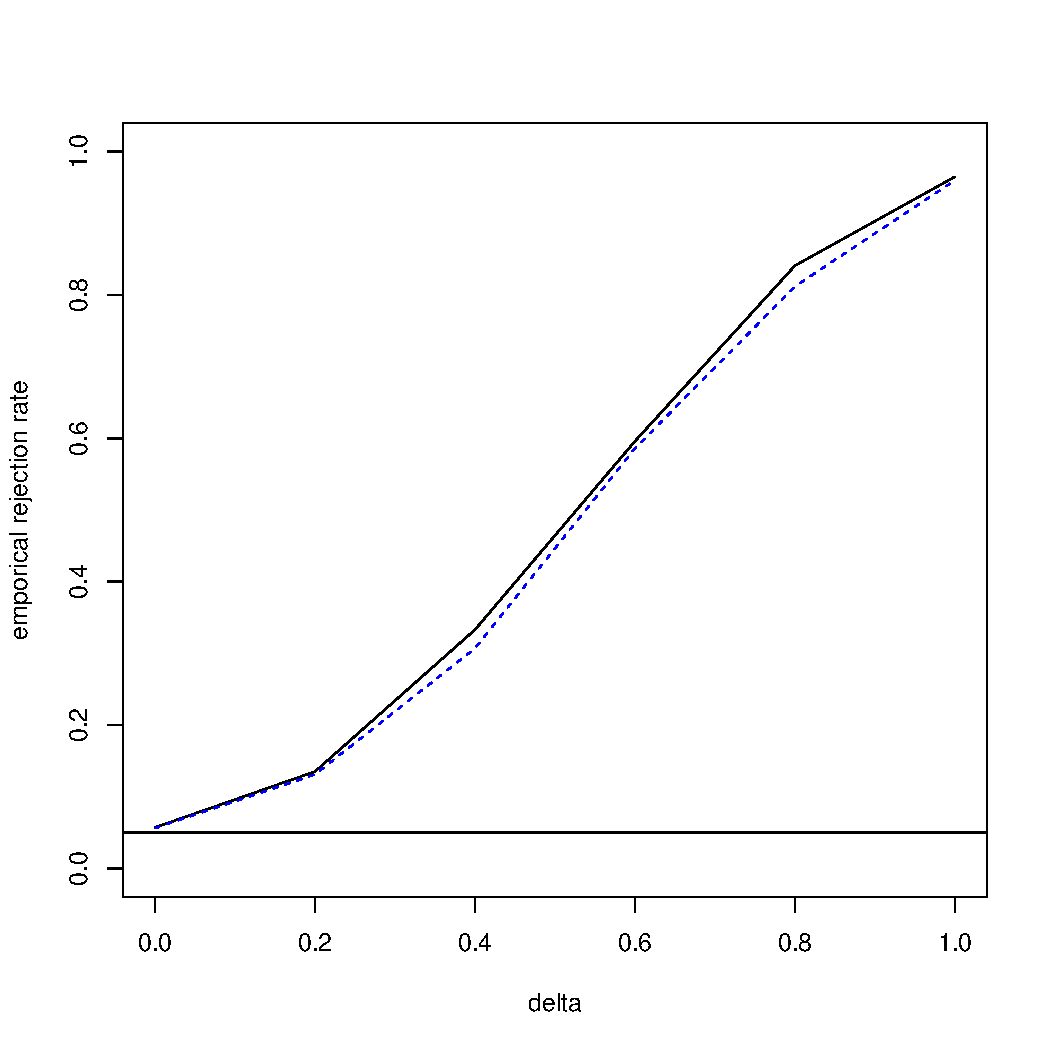
\includegraphics[width=\maxwidth]{figure/hypo-twosample-power-1} 
\begin{kframe}\begin{alltt}
\hlcom{## Cauchy distribuion}
\hlstd{rejrate} \hlkwb{<-} \hlkwd{sapply}\hlstd{(delta,} \hlkwa{function}\hlstd{(}\hlkwc{x}\hlstd{)} \hlkwd{empRejRate}\hlstd{(nrep, n, rcauchy, x))}
\hlkwd{plot}\hlstd{(delta, rejrate[}\hlstr{"t"}\hlstd{, ],} \hlkwc{type} \hlstd{=} \hlstr{"l"}\hlstd{,} \hlkwc{ylab} \hlstd{=} \hlstr{"emporical rejection rate"}\hlstd{,} \hlkwc{ylim} \hlstd{=} \hlkwd{c}\hlstd{(}\hlnum{0}\hlstd{,} \hlnum{1}\hlstd{))}
\hlkwd{lines}\hlstd{(delta, rejrate[}\hlstr{"wilcox"}\hlstd{, ],} \hlkwc{lty} \hlstd{=} \hlnum{2}\hlstd{,} \hlkwc{col} \hlstd{=} \hlstr{"blue"}\hlstd{)}
\hlkwd{abline}\hlstd{(}\hlnum{.05}\hlstd{,} \hlnum{0}\hlstd{)}
\end{alltt}
\end{kframe}
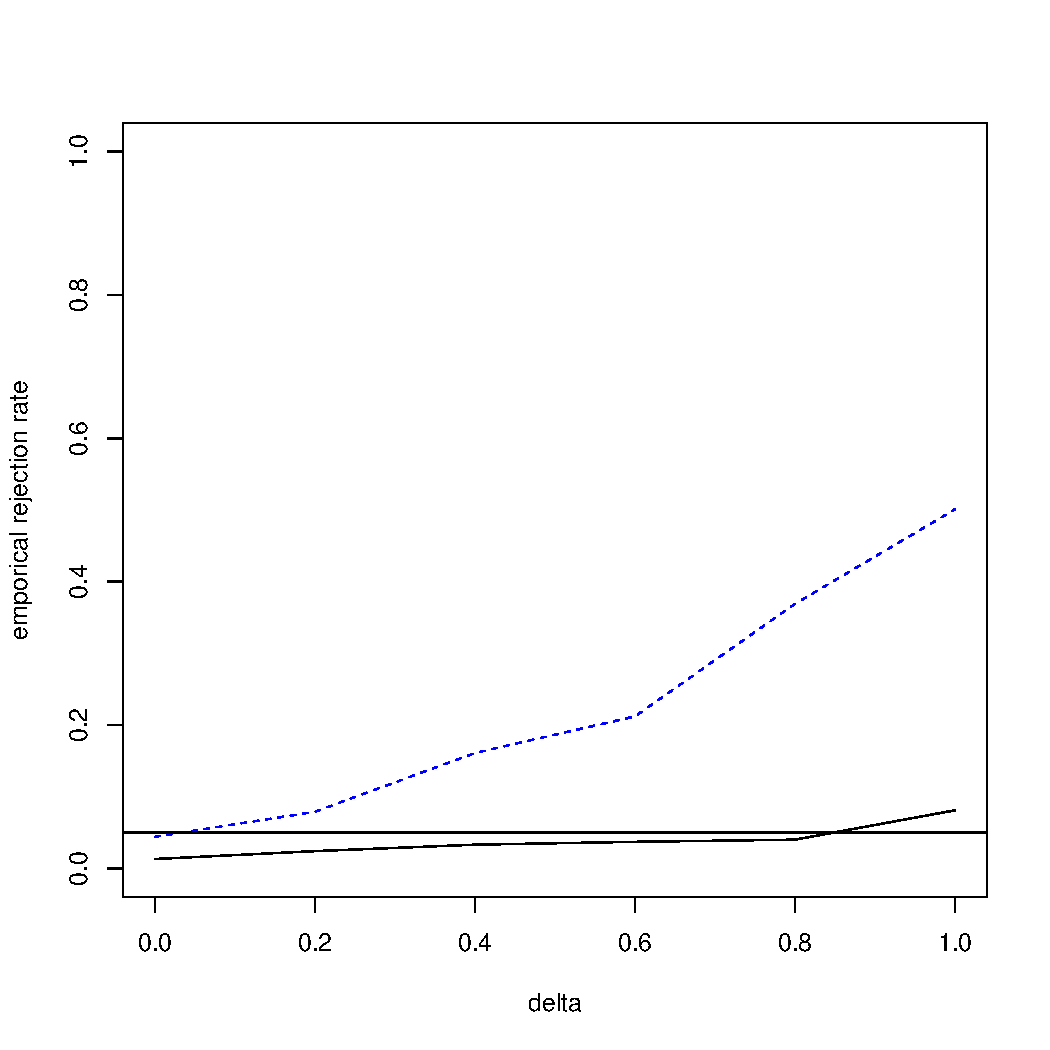
\includegraphics[width=\maxwidth]{figure/hypo-twosample-power-2} 
\end{knitrout}

Sometimes, we don't need to resort to tests based on large sample
theory. Consider the setting where we compare the two arms of
treatment in a clinical trial: treatment versus placebo. Suppose that
we want to show that the treatment leads to an increase in an outcome
of interest. Let $\mu_0$ and $\mu_1$ denote the mean of the outcome
under placebo and treatment, respectively. The hypotheses to be tested
are
\[
  H_0: \mu_1 = \mu_0,
  \quad \mbox{vs} \quad
  H_1: \mu_1 > \mu_0.
\]


Under $H_0$, the labels of the treatment arms are exchangeable.
Consider test statistics $T$, the difference in the two sample means.
\begin{knitrout}
\definecolor{shadecolor}{rgb}{0.969, 0.969, 0.969}\color{fgcolor}\begin{kframe}
\begin{alltt}
\hlstd{xpooled} \hlkwb{<-} \hlkwd{c}\hlstd{(x1, x2)}
\hlstd{xperm} \hlkwb{<-} \hlkwd{sample}\hlstd{(xpooled,} \hlkwc{size} \hlstd{=} \hlkwd{length}\hlstd{(xpooled),} \hlkwc{replace} \hlstd{=} \hlnum{FALSE}\hlstd{)}
\hlstd{xd} \hlkwb{<-}  \hlkwd{mean}\hlstd{(xperm[(n1} \hlopt{+} \hlnum{1}\hlstd{)}\hlopt{:}\hlstd{(n1} \hlopt{+} \hlstd{n2)])} \hlopt{-} \hlkwd{mean}\hlstd{(xperm[}\hlnum{1}\hlopt{:}\hlstd{n1])}
\hlcom{## put in a function}
\hlstd{myPermTest} \hlkwb{<-} \hlkwa{function}\hlstd{(}\hlkwc{x1}\hlstd{,} \hlkwc{x2}\hlstd{,} \hlkwc{nperm} \hlstd{=} \hlnum{1000}\hlstd{) \{}
    \hlstd{n1} \hlkwb{<-} \hlkwd{length}\hlstd{(x1)}
    \hlstd{n2} \hlkwb{<-} \hlkwd{length}\hlstd{(x2)}
    \hlstd{stat} \hlkwb{<-} \hlkwd{mean}\hlstd{(x2)} \hlopt{-} \hlkwd{mean}\hlstd{(x1)}
    \hlstd{xpooled} \hlkwb{<-} \hlkwd{c}\hlstd{(x1, x2)}
    \hlstd{stat.sim} \hlkwb{<-} \hlkwd{replicate}\hlstd{(nperm, \{}
        \hlstd{xperm} \hlkwb{<-} \hlkwd{sample}\hlstd{(xpooled,} \hlkwc{size} \hlstd{=} \hlkwd{length}\hlstd{(xpooled),} \hlkwc{replace} \hlstd{=} \hlnum{FALSE}\hlstd{)}
        \hlstd{xd} \hlkwb{<-} \hlkwd{mean}\hlstd{(xperm[(n1} \hlopt{+} \hlnum{1}\hlstd{)}\hlopt{:}\hlstd{(n1} \hlopt{+} \hlstd{n2)])} \hlopt{-} \hlkwd{mean}\hlstd{(xperm[}\hlnum{1}\hlopt{:}\hlstd{n1])}
    \hlstd{\})}
    \hlstd{p.value}  \hlkwb{<-} \hlkwd{mean}\hlstd{(stat.sim} \hlopt{>=} \hlstd{stat)}
    \hlstd{p.value}
\hlstd{\}}

\hlstd{delta} \hlkwb{<-} \hlnum{1}
\hlstd{x1} \hlkwb{<-} \hlkwd{rgamma}\hlstd{(n,} \hlkwc{shape} \hlstd{=} \hlnum{2}\hlstd{,} \hlkwc{scale} \hlstd{=} \hlnum{2}\hlstd{)}
\hlstd{x2} \hlkwb{<-} \hlkwd{rgamma}\hlstd{(n,} \hlkwc{shape} \hlstd{=} \hlnum{2}\hlstd{,} \hlkwc{scale} \hlstd{=} \hlnum{2}\hlstd{)} \hlopt{+} \hlstd{delta}
\hlkwd{myPermTest}\hlstd{(x1, x2)}
\end{alltt}
\begin{verbatim}
## [1] 0.12
\end{verbatim}
\begin{alltt}
\hlcom{## try a simulation study}
\hlstd{do1rep} \hlkwb{<-} \hlkwa{function}\hlstd{(}\hlkwc{n}\hlstd{,} \hlkwc{datagen}\hlstd{,} \hlkwc{delta} \hlstd{=} \hlnum{0}\hlstd{) \{}
    \hlstd{x1} \hlkwb{<-} \hlkwd{datagen}\hlstd{(n)}
    \hlstd{x2} \hlkwb{<-} \hlkwd{datagen}\hlstd{(n)} \hlopt{+} \hlstd{delta}
    \hlkwd{myPermTest}\hlstd{(x1, x2)}
\hlstd{\}}

\hlstd{sim} \hlkwb{<-} \hlkwd{replicate}\hlstd{(}\hlnum{200}\hlstd{,} \hlkwd{do1rep}\hlstd{(n, rnorm,} \hlkwc{delta} \hlstd{=} \hlnum{.5}\hlstd{))}
\hlkwd{mean}\hlstd{(sim} \hlopt{<} \hlnum{.05}\hlstd{)}
\end{alltt}
\begin{verbatim}
## [1] 0.645
\end{verbatim}
\begin{alltt}
\hlstd{sim} \hlkwb{<-} \hlkwd{replicate}\hlstd{(}\hlnum{200}\hlstd{,} \hlkwd{do1rep}\hlstd{(n, rcauchy,} \hlkwc{delta} \hlstd{=} \hlnum{1}\hlstd{))}
\hlkwd{mean}\hlstd{(sim} \hlopt{<} \hlnum{.05}\hlstd{)}
\end{alltt}
\begin{verbatim}
## [1] 0.16
\end{verbatim}
\end{kframe}
\end{knitrout}


We can test on data generated from a distribution with flexible
shapes, the generalized Tukey's lambda family, which is defined in
terms of the inverse of the distribution function.
\begin{knitrout}
\definecolor{shadecolor}{rgb}{0.969, 0.969, 0.969}\color{fgcolor}\begin{kframe}
\begin{alltt}
\hlstd{rgtl} \hlkwb{<-} \hlkwa{function}\hlstd{(}\hlkwc{n}\hlstd{,} \hlkwc{lambda1} \hlstd{=} \hlnum{0}\hlstd{,} \hlkwc{lambda2} \hlstd{=} \hlnum{1}\hlstd{,} \hlkwc{lambda3} \hlstd{=} \hlnum{0}\hlstd{,} \hlkwc{lambda4} \hlstd{=} \hlnum{1}\hlstd{) \{}
    \hlstd{u} \hlkwb{<-} \hlkwd{runif}\hlstd{(n)}
    \hlstd{lambda1} \hlopt{+} \hlstd{(u} \hlopt{^} \hlstd{lambda3} \hlopt{-} \hlstd{(}\hlnum{1} \hlopt{-} \hlstd{u)} \hlopt{^} \hlstd{lambda4)} \hlopt{/} \hlstd{lambda2}
\hlstd{\}}

\hlstd{sim} \hlkwb{<-} \hlkwd{replicate}\hlstd{(}\hlnum{200}\hlstd{,}
                 \hlkwd{do1rep}\hlstd{(n,}
                        \hlkwa{function}\hlstd{(}\hlkwc{n}\hlstd{)} \hlkwd{rgtl}\hlstd{(n,} \hlkwc{lambda3} \hlstd{=} \hlnum{1.5}\hlstd{,} \hlkwc{lambda4} \hlstd{=} \hlnum{5.8}\hlstd{),}
                        \hlkwc{delta} \hlstd{=} \hlnum{.2}\hlstd{))}
\end{alltt}
\end{kframe}
\end{knitrout}
